\documentclass[../thesis.tex]{subfiles}

%!TeX spellcheck = en-GB

% chktex-file 18

\begin{document}

\chapter{Results}
\label{chap:results}

For all values of the control parameter,\(B\), we observed that the
nearest neighbour distributions deviate from both the Poisson and Wigner distributions.
We propose the following hypothesis: the obtained nearest neighbour distributions
can be seen as a linear superposition of the
Poisson and Wigner distributions:
\[
  P(s) = \alpha P_P(s) + (1-\alpha) P_W(s).
\]

This hypothesis is rooted in the fact that the classical counterpart of our system
has an interplay between regular and chaotic motion clearly illustrated by the Poincaré
sections in figures~\ref{fig:ponicare-sections}~\cite{Baran1998}.
In this way we consider that for a range of energies of the classical system,
the phase space ratio of the volumes of chaotic and regular trajectories is
reflected in the the superposition of Wigner and Poisson distributions.

Thus, a system with an integrable classical counterpart will have \({\alpha=1}\),
corresponding to the Poisson distribution, while a fully chaotic
system will have \(\alpha=0\) corresponding to the Wigner distribution. For
a system which has balanced contributions to the phase space volume both from
the regular and chaotic trajectories, we expect the Poisson and Wigner distributions
to equally contribute to \(P(s)\).

For the fixed value of the non-integrability parameter of \(B=0.55\) we observe that
with the increase of energy, the phase space fills with tori up to a energy of
around \(E=600\) (in units of harmonic oscillator energy) and after that the chaotic trajectories begin to fill
the phase space. We can say that globally, for an energy range \(\Delta E \leq 600\),
the phase space is characterised by an increase of regular trajectories as the
energy increases. If we now consider the quantum counterpart of the system, we
can use \(\alpha \) as a measure of the closeness to the Poisson distribution.
As we can see in figures~\ref{fig:fit-b0.55n260-me100-120} and~\ref{fig:fit-b0.55n260-me150-180.3}
with the increase of the energy interval \(\alpha \) increases from \(0.493\) at
\(\Delta E \approx 100 \) to \(0.876\) at \(\Delta E \approx 180 \).

Thus, at least for a fixed value of $B$, we can observe a correlation between
the tori volume in phase space and \(\alpha \), the superposition coefficient.

\begin{figure}
\centering
\begin{subfigure}{0.49\textwidth}
  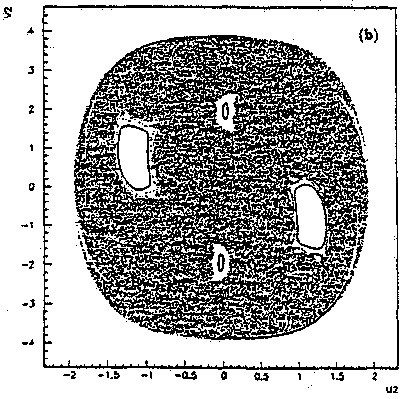
\includegraphics{ponicare-sections-e_30}  % chktex 36
\label{fig:ponicare-sections-e_30}
\end{subfigure}
\begin{subfigure}{0.49\textwidth}
  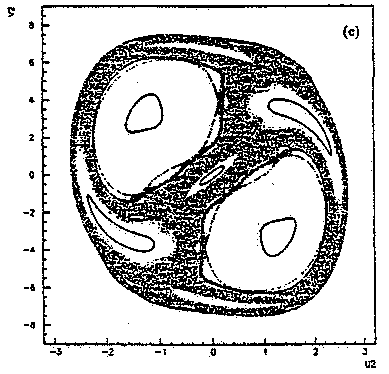
\includegraphics{ponicare-sections-e_120}  % chktex 36
\label{fig:ponicare-sections-e_120}
\end{subfigure}

\begin{subfigure}{0.49\textwidth}
  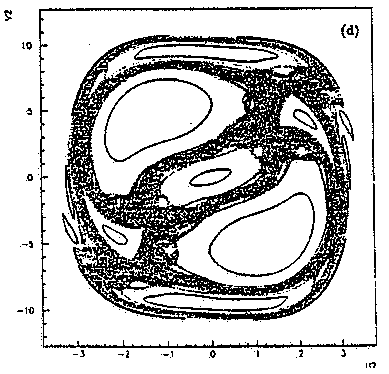
\includegraphics{ponicare-sections-e_240}  % chktex 36
\label{fig:ponicare-sections-e_240}
\end{subfigure}
\begin{subfigure}{0.49\textwidth}
  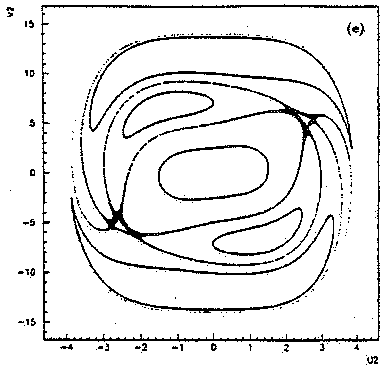
\includegraphics{ponicare-sections-e_400}  % chktex 36
\label{fig:ponicare-sections-e_400}
\end{subfigure}

\begin{subfigure}{0.49\textwidth}
  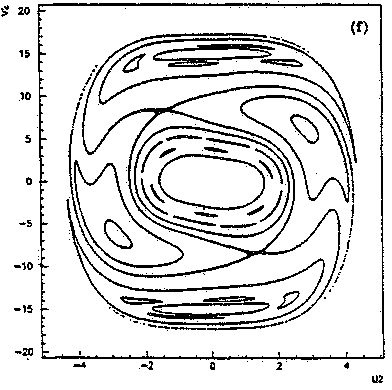
\includegraphics{ponicare-sections-e_600}  % chktex 36
\label{fig:ponicare-sections-e_600}
\end{subfigure}
\begin{subfigure}{0.49\textwidth}
  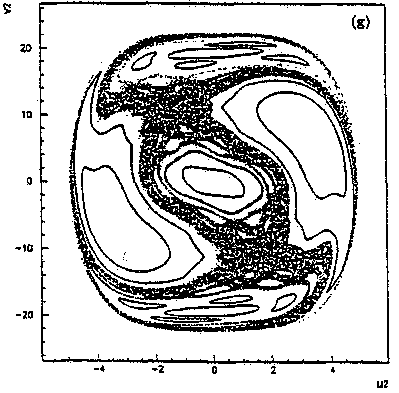
\includegraphics{ponicare-sections-e_1000}  % chktex 36
\label{fig:ponicare-sections-e_1000}
\end{subfigure}
\caption{Poincaré sections for \(B=0.55\) and \(E=30A (\text{MeV})\) (b), \({E=120A (\text{MeV})}\) (c),
\(E=240A (\text{MeV})\) (d), \(E=400A (\text{MeV})\) (e), \(E=600A (\text{MeV})\) (f), \({E=1000A (\text{MeV})}\) (g).}
\label{fig:ponicare-sections}  % chktex 24
\end{figure}

\begin{figure}
\centering
\begin{subfigure}{\textwidth}
  \includegraphics{"B0.55 D0.4 N260"/{P(s)_fit_1e-09_eps_1e-08_max_e_100.0}.pdf}  % chktex 36
\label{fig:P(s)-fit-b0.55n260-me100}
\end{subfigure}

\begin{subfigure}{\textwidth}
  \includegraphics{"B0.55 D0.4 N260"/{P(s)_fit_1e-09_eps_1e-08_max_e_120.0}.pdf}  % chktex 36
\label{fig:P(s)-fit-b0.55n260-me120}
\end{subfigure}
\caption{\(P(s)\) for \(B=0.55, D=0.4, N=260\) and \(\Delta E_{max}=100, 120\)}
\label{fig:fit-b0.55n260-me100-120}  % chktex 24
\end{figure}

\begin{figure}
\centering
\begin{subfigure}{\textwidth}
  \includegraphics{"B0.55 D0.4 N260"/{P(s)_fit_1e-09_eps_1e-08_max_e_150.0}.pdf}  % chktex 36
\label{fig:P(s)-fit-b0.55n260-me150}
\end{subfigure}

\begin{subfigure}{\textwidth}
  \includegraphics{"B0.55 D0.4 N260"/P(s)_fit_1e-09_eps_1e-08}  % chktex 36
  \label{fig:P(s)-fit-b0.55n260}  % chktex 24
\end{subfigure}
\caption{\(P(s)\) for \(B=0.55, D=0.4, N=260\) and \(\Delta E_{max}=150, 180.3\)}
\label{fig:fit-b0.55n260-me150-180.3}  % chktex 24
\end{figure}

\clearpage

Looking at other values for \(B\) such as \(B=0.2\) and \(B=0.63\), we observe
that \(P(s)\) gets closer to a Poisson distribution with the increase of energy
(see~\cref{fig:fit-b0.2n260,fig:fit-b0.63n260,fig:fit-b0.2n260-me100,fig:fit-b0.63n260-me100}).
This global feature of the system can be observed on the entire interval from
\(B=0.01\) to \(B=0.63\). In order to emphasise this, we plot \(\alpha \)
as a function of \(\Delta E\)
(see~\cref{fig:alpha-e-b0.1-0.15-0.2,fig:alpha-e-b0.25-0.3-0.35,fig:alpha-e-b0.4-0.45-0.5,fig:alpha-e-b0.55-0.6-0.63}).

This remarkable behaviour can be viewed as consequence of the interplay of the
third and fourth order terms in the Hamiltonian. The third order terms, which
consist in the non-integrable part of the Hamiltonian and can be considered as
contributing to the apparition of chaotic trajectories.

\begin{figure}
\centering
  \begin{subfigure}{\textwidth}
    \includegraphics{"B0.2 D0.4 N260"/P(s)_fit_1e-09_eps_1e-08}  % chktex 36
    \label{fig:P(s)-fit-b0.2n260}  % chktex 24
  \end{subfigure}

  \begin{subfigure}{\textwidth}
    \includegraphics{"B0.2 D0.4 N260"/I(s)_fit}  % chktex 36
  \label{fig:I(s)-fit-b0.2n260}  % chktex 24
  \end{subfigure}
  \caption{\(P(s), I(s)\) for \(B=0.2, D=0.4, N=260\)}
  \label{fig:fit-b0.2n260}  % chktex 24
\end{figure}

\begin{figure}
\centering
  \begin{subfigure}{\textwidth}
    \includegraphics{"B0.63 D0.4 N260"/P(s)_fit_1e-09_eps_1e-08}  % chktex 36
    \label{fig:P(s)-fit-b0.63n260}  % chktex 24
  \end{subfigure}

  \begin{subfigure}{\textwidth}
    \includegraphics{"B0.63 D0.4 N260"/I(s)_fit}  % chktex 36
  \label{fig:I(s)-fit-b0.63n260}  % chktex 24
  \end{subfigure}
  \caption{\(P(s), I(s)\) for \(B=0.63, D=0.4, N=260\)}
  \label{fig:fit-b0.63n260}  % chktex 24
\end{figure}

\begin{figure}
\centering
\begin{subfigure}{\textwidth}
  \includegraphics{"B0.2 D0.4 N260"/{P(s)_fit_1e-09_eps_1e-08_max_e_100.0}.pdf}  % chktex 36
\label{fig:P(s)-fit-b0.2n260-me100}
\end{subfigure}

\begin{subfigure}{\textwidth}
  \includegraphics{"B0.2 D0.4 N260"/{I(s)_fit_max_e_100.0}.pdf}  % chktex 36
  \label{fig:I(s)-fit-b0.2n260-me100}  % chktex 24
\end{subfigure}
\caption{\(B=0.2, D=0.4, N=260, \Delta E_{max}=100\)}
\label{fig:fit-b0.2n260-me100}
\end{figure}

\begin{figure}
\centering
\begin{subfigure}{\textwidth}
  \includegraphics{"B0.63 D0.4 N260"/{P(s)_fit_1e-09_eps_1e-08_max_e_100.0}.pdf}  % chktex 36
\label{fig:P(s)-fit-b0.63n260-me100}
\end{subfigure}

\begin{subfigure}{\textwidth}
  \includegraphics{"B0.63 D0.4 N260"/{I(s)_fit_max_e_100.0}.pdf}  % chktex 36
  \label{fig:I(s)-fit-b0.63n260-me100}  % chktex 24
\end{subfigure}
\caption{\(B=0.63, D=0.4, N=260, \Delta E_{max}=100\)}
\label{fig:fit-b0.63n260-me100}
\end{figure}

% alpha(deltaE)

\begin{figure}
  \includegraphics{{"alpha_e_B[0.1, 0.15, 0.2]"_N[260]}.pdf}  % chktex 36
  \caption{\(B=0.1, 0.15, 0.2,\; N=260\)}
\label{fig:alpha-e-b0.1-0.15-0.2}
\end{figure}

\begin{figure}
  \includegraphics{{"alpha_e_B[0.25, 0.3, 0.35]"_N[260]}.pdf}  % chktex 36
  \caption{\(B=0.25, 0.3, 0.35,\; N=260\)}  % replace
\label{fig:alpha-e-b0.25-0.3-0.35}
\end{figure}

\begin{figure}
  \includegraphics{{"alpha_e_B[0.4, 0.45, 0.5]"_N[260]}.pdf}  % chktex 36
  \caption{\(B=0.4, 0.45, 0.5,\; N=260\)}  % replace
\label{fig:alpha-e-b0.4-0.45-0.5}
\end{figure}

\begin{figure}
  \includegraphics{{"alpha_e_B[0.55, 0.6, 0.63]"_N[260]}.pdf}  % chktex 36
  \caption{\(B=0.55, 0.6, 0.63,\; N=260\)}   % replace
\label{fig:alpha-e-b0.55-0.6-0.63}
\end{figure}

An other global characteristic of the system can be revealed by studying the
dependence of \(\alpha \) on the non-integrability parameter $B$.
In figure~\ref{fig:alpha-n220-240-260} \(\alpha(B)\) is plotted for
different values of $N$. The value of $N$ determines both the stability
of the values and the maximum energy interval. Indeed, since our method implies the
truncation of the Hilbert space, we restrict the number of considered energy
levels with the stability criterion.

As with the above case of \(\alpha(\Delta E)\), we can reduce the energy interval
by considering only the energy levels up to a given value. In figures~\ref{fig:alpha-n260-me100-120-140}
and~\ref{fig:alpha-n260-me140-160-0} we can see that the shape of \(\alpha(B)\)
for \(N=260\) remains qualitatively the same when we consider different
values for the maximum energy interval. We can observe that as we increase
the energy the values of \(\alpha \) globally rise, as expected from the
previous plots.

An other qualitative test of our data implies checking how the values of
\(\alpha \) change when we consider different values for \(N\), in this
case \(N=220, 240, 260\) and different energy intervals. By considering
multiple values for $N$ we can check the stability of the energy levels
within a given interval provided that the respective interval is less than
the maximum energy interval for all $N$.
In~\cref{fig:alpha-n220-240-260-me100,fig:alpha-n220-240-260-me120,fig:alpha-n220-240-260-me140}
we can see that indeed the energy levels
are stable as the values of \(\alpha \) barely change.

% alpha(B)

\begin{figure}
  \includegraphics{"alpha_N[220, 240, 260]".pdf}  % chktex 36
  \caption{\(N=220, 240, 260\)}
\label{fig:alpha-n220-240-260}
\end{figure}

\begin{figure}
  \includegraphics{{alpha_N[260]_max_e_"[100.0, 120.0, 140.0]"}.pdf}  % chktex 36
  \caption{\(N=260,\; \Delta E_{max} \approx 100, 120, 140\)}
\label{fig:alpha-n260-me100-120-140}
\end{figure}

\begin{figure}
  \includegraphics{{alpha_N[260]_max_e_"[140.0, 160.0, 0.0]"}.pdf}  % chktex 36
  \caption{\(N=260,\; \Delta E_{max} \approx 140, 160, 190.305\)}
\label{fig:alpha-n260-me140-160-0}
\end{figure}

\begin{figure}
  \includegraphics{{"alpha_N[220, 240, 260]"_max_e_[100.0]}.pdf}  % chktex 36
  \caption{\(N=220, 240, 260,\; \Delta E_{max} \approx 100\)}
\label{fig:alpha-n220-240-260-me100}
\end{figure}

\begin{figure}
  \includegraphics{{"alpha_N[220, 240, 260]"_max_e_[120.0]}.pdf}  % chktex 36
  \caption{\(N=220, 240, 260,\; \Delta E_{max} \approx 120\)}
\label{fig:alpha-n220-240-260-me120}
\end{figure}

\begin{figure}
  \includegraphics{{"alpha_N[220, 240, 260]"_max_e_[140.0]}.pdf}  % chktex 36
  \caption{\(N=220, 240, 260,\; \Delta E_{max} \approx 140\)}
\label{fig:alpha-n220-240-260-me140}
\end{figure}



\end{document}
